\documentclass[12pt,a4paper]{article}

\usepackage[utf8]{inputenc}
\usepackage[T1]{fontenc}
\usepackage{lmodern}
\usepackage{amsmath, amssymb}
\usepackage{graphicx}
\usepackage{caption}
\usepackage{subcaption}
\usepackage{booktabs}
\usepackage{geometry}
\usepackage{natbib}
\usepackage{setspace}
\usepackage{hyperref}

\geometry{left=3cm, right=2cm, top=2cm, bottom=2cm}
\onehalfspacing

\begin{document}


\subsection{Life Cycle Assessment (LCA) Method}
The LCA method calculates emissions throughout the entire life cycle of a product or service, from production to disposal. This model captures emissions from every stage of the supply chain and provides a comprehensive assessment of indirect emissions.

The carbon footprint for a single industry using the LCA approach is:
\[
fp_h = q_h \cdot \text{LCA}_j
\]
where \(q_h\) is the quantity consumed by household \(h\), and \(\text{LCA}_j\) represents the life cycle emissions per unit in industry \(j\).


\subsubsection{Methodology for Household Carbon Footprint Calculation based on LCA approach}

The methodology developed by Peng et al. (2021) provides a comprehensive framework for calculating household carbon footprints by integrating life-cycle assessment (LCA) approaches. This framework accounts for both carbon emissions and sequestration from various household activities, including consumption and production, using survey data. It employs three primary LCA methods: (1) \textit{Process LCA}, which evaluates emissions from agricultural and livestock-related processes, capturing material inputs like fertilizers and operational activities; (2) \textit{Input–Output LCA}, applied to household consumption activities such as energy, food, housing, and transportation; and (3) \textit{Hybrid LCA}, which combines process and input-output methods to assess afforestation activities and durable goods like clothing. The methodology categorizes household activities into specific domains, including direct energy consumption, living consumption (short-lived and durable goods), agricultural activities (emissions from material inputs and sequestration from biomass growth), afforestation (carbon sequestration from tree plantations such as citrus farming), and livestock raising (emissions from fodder preparation, livestock growth, and manure management). The total carbon footprint is expressed as the sum of emissions and sequestration across these domains, incorporating emission factors and material inputs derived from IPCC guidelines and regional data. 
\subsubsection*{Overall Carbon Footprint}
\begin{equation}
CF_i = \sum_{n} E_{in} + \sum_{m} S_{im}
\end{equation}
where $CF_i$ represents the Carbon footprint of household $i$, $E_{in}$ is the annual carbon emissions of household $i$ in category $n$ and $S_{im}$ is the annual carbon sequestration of household $i$ in category $m$.


\subsubsection*{Carbon Emissions from Direct Energy Consumption}
\begin{equation}
E_{id} = \sum_d (F_{id} \cdot EF_d)
\end{equation}
\begin{equation}
EF_d = OX_d \cdot \left(C_{o,d} \cdot \frac{12}{44} + C_{h,d} \cdot \frac{12}{16}\right) \cdot H_d \cdot 10^{-9}
\end{equation}

where $E_{id}$ is the carbon emissions from direct fuel consumption, $F_{id}$ is the fuel consumption of household $i$ for fuel type $d$, $EF_d$ is the emission factor of fuel $d$, $OX_d$ is the oxygenation efficiency (assumed 100\%), $C_{o,d}$ and $C_{h,d}$ are the CO$_2$ and CH$_4$ emission factors, and $H_d$ is the net calorific value of the fuel.


\subsubsection*{Carbon Emissions from Living Consumption}
\begin{equation}
E_{if} = \sum_f (EF_f \cdot C_{if})
\end{equation}
\begin{equation}
E_{ij} = \sum_j \frac{(EF_j \cdot C_{ij})}{L_j}
\end{equation}
where: $E_{if}$ and $E_{ij}$ are the carbon emissions from short-lived and durable consumer products, $C_{if}$ and $C_{ij}$ are the amounts of consumed material, and $L_j$ is the lifetime of durable consumer product $j$.


\subsubsection*{Carbon Footprint in Agricultural Activities}
\begin{equation}
CF_{ia} = \sum_a (EF_a \cdot M_{ia}) + \sum_t (EF_t \cdot FS_{ia}) + \sum_v (B_v \cdot 0.475)
\end{equation}
where: $CF_{ia}$ is the carbon footprint from agricultural activities, $EF_a$ and $EF_t$ are the emission factors for materials and field operations, $M_{ia}$ is the material input, $FS_{ia}$ is the field size, and $B_v$ is the biomass produced.


\subsubsection*{Carbon Sequestration from Afforestation}
\begin{equation}
S_{iaf} = FS_{iaf} \cdot CS_{\text{citrus}}
\end{equation}
where: $S_{iaf}$ is the carbon sequestration from afforestation, $FS_{iaf}$ is the field size for afforestation, and $CS_{\text{citrus}}$ is the carbon stock of citrus trees.


\subsubsection*{Carbon Emissions from Livestock Raising}
\begin{equation}
E_{il} = \sum_f (EF_{if} \cdot F_{if}) + \sum_l (EF_{il} \cdot N_{il})
\end{equation}
where: $E_{il}$ is the carbon emissions from livestock raising, $EF_{if}$ and $EF_{il}$ are the emission factors for fodder and livestock, $F_{if}$ is the fodder consumption, and $N_{il}$ is the number of livestock.



\subsubsection*{Aggregate Formula for Household Carbon Footprint}

The total carbon footprint ($CF_{\text{total}}$) of a household is the sum of emissions and sequestration from all relevant activities, including direct energy consumption, living consumption, agricultural activities, afforestation, and livestock raising:

\begin{align}
CF_{\text{total}} = & \underbrace{\sum_d \left(F_{id} \cdot EF_d\right)}_{\text{Direct energy consumption}} + 
\underbrace{\sum_f \left(EF_f \cdot C_{if}\right) + \sum_j \frac{\left(EF_j \cdot C_{ij}\right)}{L_j}}_{\text{Living consumption}} \nonumber \\
& + \underbrace{\sum_a \left(EF_a \cdot M_{ia}\right) + \sum_t \left(EF_t \cdot FS_{ia}\right) + \sum_v \left(B_v \cdot 0.475\right)}_{\text{Agricultural activities}} \nonumber \\
& - \underbrace{\sum_{iaf} \left(FS_{iaf} \cdot CS_{\text{citrus}}\right)}_{\text{Afforestation}} +
\underbrace{\sum_f \left(EF_{if} \cdot F_{if}\right) + \sum_l \left(EF_{il} \cdot N_{il}\right)}_{\text{Livestock raising}}
\end{align}


The total household carbon footprint is denoted by $CF_{\text{total}}$. Fuel consumption for fuel type $d$ is represented by $F_{id}$, and the emission factor of fuel $d$ is denoted by $EF_d$. The amount of consumed materials for short-lived ($f$) and durable products ($j$) is represented by $C_{if}$ and $C_{ij}$, respectively, with the lifetime of durable product $j$ given by $L_j$. The emission factors for short-lived and durable products are represented by $EF_f$ and $EF_j$, respectively. The material input for agricultural activity $a$ is denoted by $M_{ia}$, while the emission factors for agricultural materials and field operations are given by $EF_a$ and $EF_t$. The field size for agricultural activities is represented by $FS_{ia}$, and the biomass produced is denoted by $B_v$. The field size for afforestation is represented by $FS_{iaf}$, while the carbon stock of citrus trees is given by $CS_{\text{citrus}}$. Fodder consumption for livestock is denoted by $F_{if}$, and the number of livestock is represented by $N_{il}$. The emission factors for fodder and livestock are represented by $EF_{if}$ and $EF_{il}$, respectively.

\section{LCA Illustration}

An integrated life cycle assessment (LCA) illustration highlights the relative contributions of household activities to carbon footprints by combining insights from Peng et al. (2021), Sala et al. (2014), and Matthews et al. (2008). Direct fuel use, including heating fuels and private vehicle fuels, accounts for approximately 20\%–30\% of total household greenhouse gas emissions. Living consumption, encompassing short-lived goods, services, and food, represents 50\%–60\% of total emissions. Within this category, the Mediterranean diet contributes approximately 2–3 tCO2e per capita annually, with red meat and dairy products responsible for over 60\% of diet-related emissions despite contributing a smaller share of caloric intake. Cereals, fruits, and vegetables, staples of the Mediterranean diet, contribute a relatively minor portion of dietary greenhouse gas emissions. Durable goods, such as furniture and household appliances, contribute an additional 5\%–10\% of emissions over their service life. The combined evidence demonstrates that focusing solely on direct energy use or Tier 1 emissions substantially underestimates the total carbon footprint of household consumption, as supply chain and embodied emissions account for the majority of impacts. This illustration is important because it emphasizes the need for comprehensive, activity-based accounting of household emissions to inform effective mitigation strategies and to enable comparison with input-output or equilibrium-based models.
\begin{figure}[h]
\centering
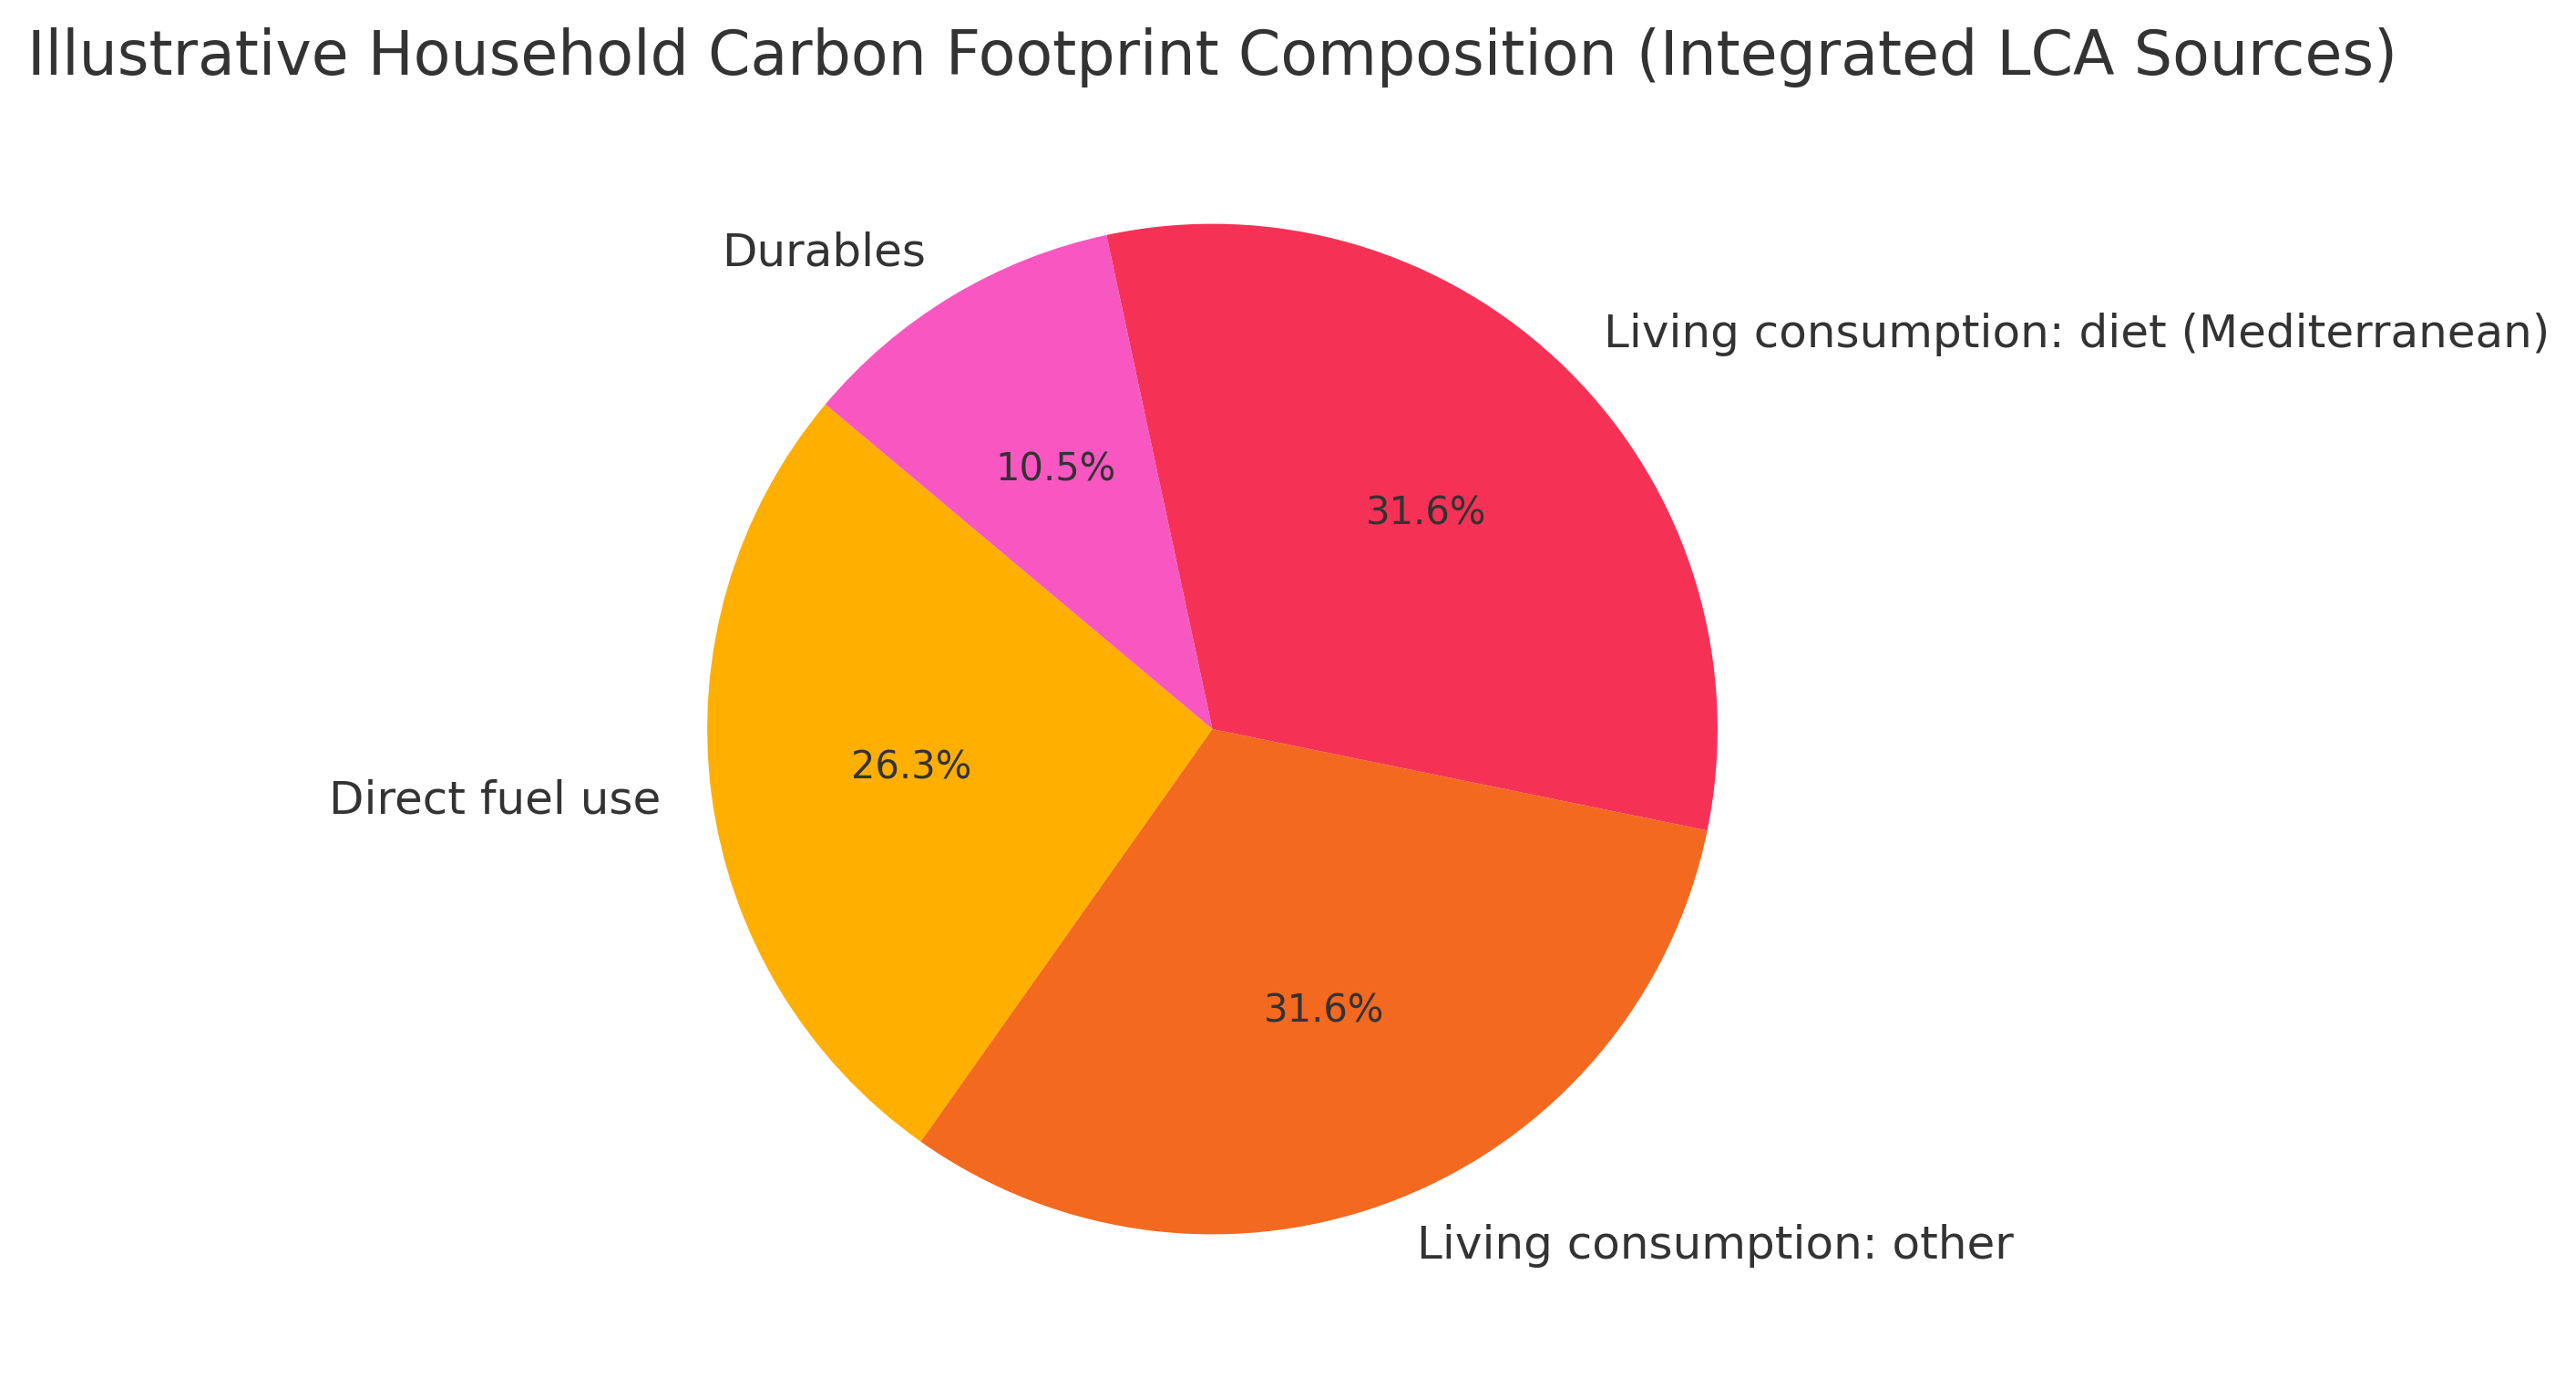
\includegraphics[width=0.8\linewidth]{LCA_pie_chart.png}
\caption{Relative contributions of household activities to carbon footprints}
\end{figure}

\section{Illustration of LCA with Comparative Insights from EEIOA}

Life cycle assessment (LCA) and environmentally extended input--output analysis (EEIOA) are two established methods for quantifying the carbon footprint of household consumption. While both approaches aim to capture direct and indirect greenhouse gas (GHG) emissions, they differ significantly in scope, resolution, and attribution of emissions. This section illustrates the application of LCA to household carbon footprints, integrating insights from Steubing et al. (2022), who compare LCA-based carbon footprints with those derived from EEIOA databases.

In the LCA approach, household carbon footprints are computed by summing emissions across all relevant activities and life cycle stages. The total household carbon footprint can be expressed as:
\begin{equation}
\text{CF}_{\text{total}} = \sum_d (F_{id} \cdot EF_d) 
+ \sum_f (C_{if} \cdot EF_f) 
+ \sum_j \left( \frac{C_{ij} \cdot EF_j}{L_j} \right)
+ \sum_a (M_{ia} \cdot EF_a)
- \sum_t (S_{it} \cdot CS_t)
\end{equation}
where $F_{id}$ is the fuel consumption for fuel type $d$, $C_{if}$ is the consumption of short-lived goods $f$, $C_{ij}$ is the consumption of durable goods $j$ with lifespan $L_j$, $M_{ia}$ is the material input for agricultural activity $a$, and $S_{it}$ is the sequestration from afforestation activity $t$. $EF$ and $CS$ denote emission factors and carbon stock, respectively.

Steubing et al. (2022) highlight that LCA-based carbon footprints typically provide a detailed, process-specific view, often including the life cycle impacts of capital goods and infrastructure. In contrast, EEIOA provides a macroeconomic perspective, covering the entire supply chain through national accounting frameworks. A key finding is that, despite theoretical expectations that EEIOA would yield higher carbon footprints due to the avoidance of truncation errors, LCA-based estimates can be higher in certain sectors. This discrepancy arises because LCA more comprehensively accounts for capital goods and specific life cycle stages, whereas EEIOA often omits the impacts of capital formation, as represented mathematically by the exclusion of gross fixed capital formation from the supply chain matrix:
\begin{equation}
\text{CF}_{\text{EEIOA}} = R (I - A)^{-1} y
\end{equation}
where $R$ is the vector of emission intensities, $A$ is the technology matrix, $I$ is the identity matrix, and $y$ is the final demand vector. In standard EEIOA practice, $y$ excludes capital goods destined for production.

Comparative analysis reveals that LCA is particularly effective in capturing emissions from long-lived assets and infrastructure-intensive activities, such as renewable energy installations, whereas EEIOA better reflects the systemic supply chain emissions associated with everyday consumption. This has critical implications for household carbon footprint assessments: neglecting either method's strengths risks underrepresenting key components of emissions. For instance, Steubing et al. (2022) report that for electricity, fossil-fuel-based power shows good alignment between LCA and EEIOA results, while renewable energy systems exhibit larger discrepancies due to the treatment of construction impacts in LCA.

Illustrating household carbon footprints using LCA not only clarifies the sources of emissions by activity and material flow but also exposes the limitations of relying on purely economic or monetary input--output models. The integrated perspective is essential for designing mitigation strategies that address both immediate consumption patterns and the long-term impacts of infrastructure and capital goods.


\end{document}


